\section{传感器}

\begin{frame}
    \frametitle{传感}
    如果我们要对自然界的信号加以记录和处理，我们应该是先把这些信号转变为电信号。这个转换的过程就叫做“\highlight{传感}”。

    执行这个过程的器件叫做\highlight{传感器}。传感器把某种物理量转变成了以电压或者电流表示的信号。

    这个信号是对现实世界物理量的“复刻”或者说“再现”。

\end{frame}

\begin{frame}
    \frametitle{传感器}
    传感器是将各种非电量（包括物理量、化学量、生物量等）按一定规律转换成便于处理和传输的另一种物理量（一般为电量）的装置。

传感器技术是利用各种功能材料实现信息检测的一门应用技术，它是检测（传感）原理、材料科学、工艺加工等三个要素的最佳结合。

传感原理是传感器工作时所依据的物理效应、化学反应和生物反应等机理，各种功能材料则是传感技术发展的物质基础，从某种意义上讲，传感器也就是能感知外界各种被测信号的功能材料。

\end{frame}

\begin{frame}
    \frametitle{传感器的组成}
    传感器（sensor）是由敏感元件和转换元件组成的一种检测装置，能感受到被测量，并能将检测和感受到的信息，按一定规律变换成为电信号（电压、电流、频率或相位）输出，以满足感知信息的传输、处理、存储、显示、记录和控制的要求。
    \bigskip

    \begin{center}
        \begin{tikzpicture}
            \draw[->] (0,0.5) -- (2,0.5) node [above,midway] {被测信息};
            \draw (2,0) rectangle (4,1) node [midway] {敏感元件};
            \draw[->,shift={(4,0)}] (0,0.5) -- (2,0.5);
            \draw[shift={(4,0)}] (2,0) rectangle (4,1) node [midway] {转换元件};
            \draw[->,shift={(8,0)}] (0,0.5) -- (2,0.5);
            \draw[shift={(8,0)}] (2,0) rectangle (5,1) node [midway] {信号调理电路};
            \draw[->,shift={(13,0)}] (0,0.5) -- (2,0.5) node [above,midway] {输出信息};
            \draw[->,shift={(7,0)}] (0,-1) -- (0,0);
            \draw[->,shift={(12.5,0)}] (0,-1) -- (0,0);
            \draw (6,-2) rectangle (13,-1) node [midway] {辅助电源电路};
        \end{tikzpicture}
    \end{center}
\end{frame}





\subsection{传感器的分类}

\begin{frame}
    \frametitle{按照测量对象进行分类}
        \begin{minipage}{0.25\linewidth}
            \begin{itemize}
                \item 温度传感器
                \item 压力传感器
                \item 位移传感器
                \item 速度传感器
                \item 湿度传感器
                \item 气体传感器
                \item $\cdots \cdots$
            \end{itemize}
        \end{minipage}\hfill
        \begin{minipage}{0.73\linewidth}
            \begin{figure}[htpb]
                \centering
                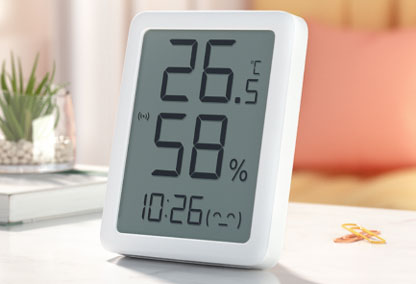
\includegraphics[height=.3\textwidth]{images/温度湿度计}
                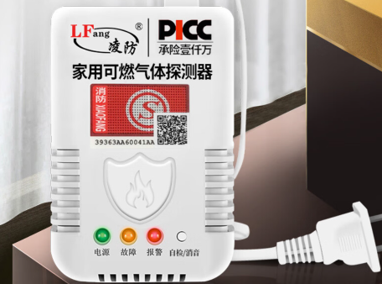
\includegraphics[height=.3\textwidth]{images/可燃气体传感器}
                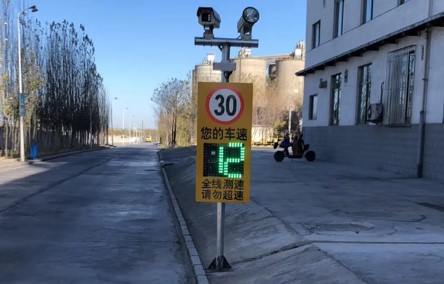
\includegraphics[height=.3\textwidth]{images/车速测量}
                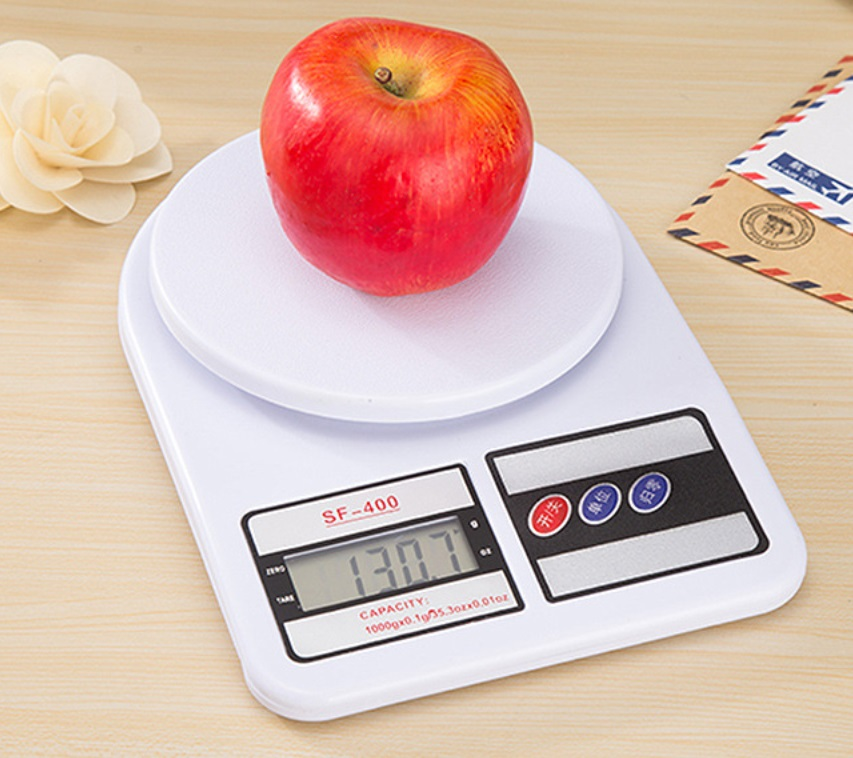
\includegraphics[width=.375\textwidth, height=.3\textwidth]{images/电子称.jpg}
            \end{figure}
        \end{minipage}
\end{frame}

\begin{frame}
    \frametitle{按照检测原理进行分类}
    \begin{itemize}
        \item {\cbf{物理传感器}}
        
        物理传感器是检测物理量的传感器。它是利用某些物理效应，把被测量的物理量转化成为便于处理的能量形式的信号的装置。

        如力传感器、声传感器、温度传感器、光传感器、电传感器、磁传感器、射线传感器
        \item {\cbf{化学传感器}}
        
        化学传感器是对各种化学物质敏感并将其浓度转换为电信号进行检测的仪器。
        \item {\cbf{生物传感器}}
        
        生物传感器是由生物敏感元件与信号转换器构成的分析装置。

        生物敏感元件的作用是识别目标物质，主要包括：抗体、酶、核酸、细胞等生物物质；也包括一些类似于生物物质的合成的物质。
    \end{itemize}
\end{frame}

\begin{frame}
    \frametitle{按照传感器的结构参数在信号变换过程中是否发生变化进行分类}
    \begin{itemize}
        \item {\cbf{物性型}}
        
        在实现信号的变换过程中，结构参数基本不变，而是依靠敏感元件材料本身物理或化学性质的变化来实现信号变换。例如利用水银的热胀冷缩现象制成水银温度计来测温；利用石英晶体的压电效应制成压电测力计等。

        \begin{itemize}
            \item 压阻式传感器（压阻效应，压阻系数改变）
            \item 光电式传感器（光电效应，光子轰击引起物体电阻率改变）
            \item 压电式传感器（压电效应，压力引起电动势改变）
            \item 热电式传感器（热电效应，温度引起电动势改变）
        \end{itemize}
        \item {\cbf{结构型}}
        
        依靠传感器结构参数的变化而将外界被测量参数转化成相应的电阻、电感、电容等物理量的变化，实现信号转换。
        \begin{itemize}
            \item 电容式传感器依靠极板间距离变化引起电容量变化；
            \item 电感式传感器依靠衔铁位移引起自感或互感变化等。
        \end{itemize}
        
    \end{itemize}
\end{frame}

\begin{frame}
    \frametitle{根据敏感元件与被测对象之间的能量关系进行分类}
    \begin{itemize}
        \item {\cbf{能量转换型}}
        
        该类传感器能将输入的非电能量转换成电能输出，传感器本身勿需外加电源，信号能量直接从被测对象取得。
        
        但由于这类传感器是被测对象与传感器之间的能量传输，必然导致被测对象状态的变化，而造成测量误差。

        \item {\cbf{能量控制型}}
        
        该类传感器在进行信号转换时，需要从外部供给辅助能源使传感器工作，并由被测量来控制外部供给能量的变化。通过测量电路将它变为电压或电流量，然后进行转换、放大，以推动指示或记录仪表。

        例如，电阻应变测量中，应变计接于电桥上，电桥工作能源由外部供给，而由于被测量变化所引起应变计的电阻变化来控制电桥的不平衡程度。
    \end{itemize}
\end{frame}


\begin{frame}
    \frametitle{自发电无线门铃\link{https://www.bilibili.com/video/av94579506}}
    \begin{figure}[htpb]
        \centering
        
\includegraphics[width=.7\linewidth]{门铃}
    \end{figure}
\end{frame}


\begin{frame}
    \frametitle{按输出信号的性质分类}
    \begin{itemize}
        \item {\cbf{模拟式传感器}}
        
        将被测非电量转换成连续变化的电压或电流。

        模拟传感器的模拟处理方式是连续的。一旦输入改变，输出也会改变。
        \item {\cbf{数字式传感器}}
        
        能直接将非电量转换为数字量，可以直接用于数字显示和计算，可直接配合计算机，具有抗干扰能力强，适宜距离传输等优点。

        数字传感器的数字处理方式是离散的。当输入更改时，系统会记录更改之前会存在延迟。此延迟的长度由“采样频率”决定，并由时钟控制。
    \end{itemize}
\end{frame}

\begin{frame}
    \frametitle{按照传感器与被测对象的关联方式进行分类}
    \begin{itemize}
        \item {\cbf{接触式}}
        
        必须接触才能有信号。如压力传感器，电位差计式传感器等。
        \item {\cbf{非接触式}}
        
        非接触化测量可以消除传感器介入而使被测量受到的影响，提高测量的准确性，同时，可使传感器的使用寿命增加。但是非接触式传感器的输出会受到被测对象与传感器之间介质或环境的影响。因此传感器标定必须在使用现场进行。例如红外测温枪、红外测温仪以及农业遥感、航空摄影均属于非接触式传感技术。
    \end{itemize}
\end{frame}

\begin{frame}
    \frametitle{按作用形式分类}
        \begin{minipage}{0.38\linewidth}
            \begin{itemize}
                \item {\cbf{主动型}}
                
                主动发出探测信号
                    \begin{itemize}
                        \item 激光雷达
                        \item 声纳
                    \end{itemize}
                \item {\cbf{被动型}}
                
                被动接收被测对象本身产生的信号
                \begin{itemize}
                    \item 红外辐射温度计
                    \item 红外摄像装置
                \end{itemize}
            \end{itemize}
        \end{minipage}\hfill
        \begin{minipage}{0.58\linewidth}
            \begin{figure}[htpb]
                \centering
                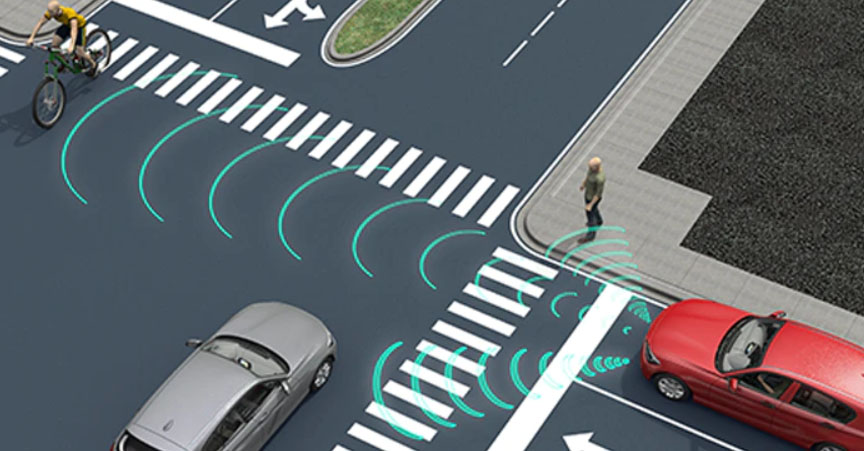
\includegraphics[width=\linewidth]{images/雷达}
            \end{figure}
        \end{minipage}
    
\end{frame}

\begin{frame}
    \frametitle{按传感器构成来分类}
    \begin{center}
        {\Large \cbf{“没有什么是一个传感器解决不了的”}}
        \bigskip

        {\Large \cbf{“如果有，就两个”}}
    \end{center}
    \begin{itemize}
      \item {\cbf{基本型传感器}}
      
      是一种最基本的单个变换装置
      \item {\cbf{组合型传感器}}
      
      是由不同单个变换装置组合而构成的传感器
      \item {\cbf{应用型传感器}}
      
      是基本型传感器或组合型传感器与其他机构组合而构成的传感器
    \end{itemize}
\end{frame}

\subsection{常用传感器}

\begin{frame}
    \frametitle{温度传感器}
    \begin{figure}[htpb]
        \centering
        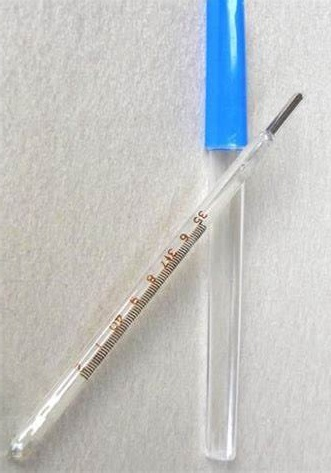
\includegraphics[height=.44\linewidth]{images/水银温度计.jpg}
        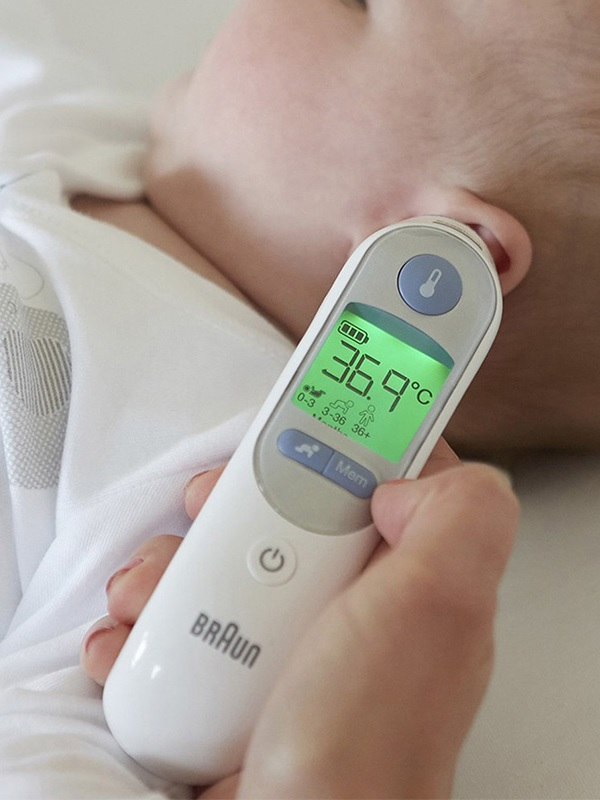
\includegraphics[height=.44\linewidth]{images/耳温枪.jpg}
        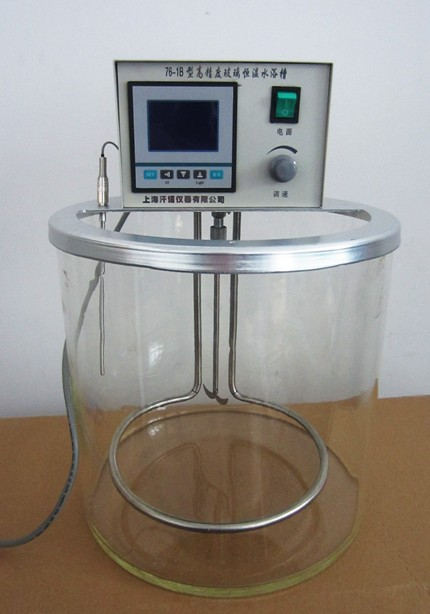
\includegraphics[height=.44\linewidth]{images/水浴锅.jpg}
    \end{figure}
\end{frame}

% 恒温水浴锅是利用传感器将水槽内水的温度转换为电阻值，输出控制信号，有效地控制电加热管的平均加热功率，使水槽内的水保持恒温。常作蒸发和恒温加热用，当被加热的物体要求受热均匀，温度不超过100℃时，可以用水浴加热。

\begin{frame}
    \frametitle{力传感器}
        \begin{minipage}{0.63\linewidth}
            \begin{figure}[htpb]
                \centering
                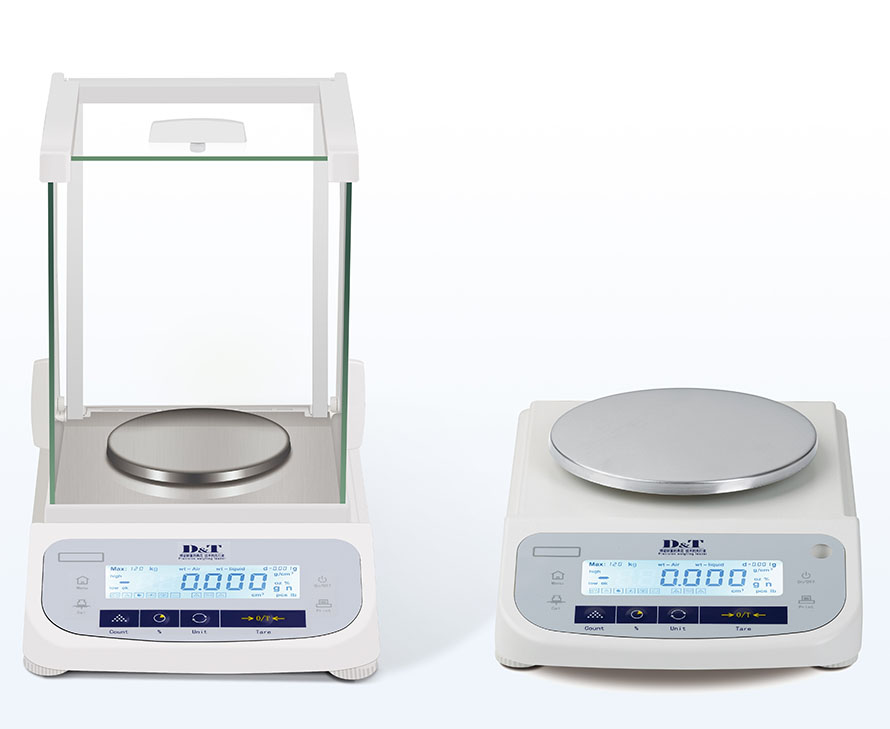
\includegraphics[height=200pt]{images/天平}
            \end{figure}
        \end{minipage}\hfill
        \begin{minipage}{0.35\linewidth}
            
            \begin{itemize}
                \item 压电式压力传感器
                \item 压阻式压力传感器
                \item 电容式压力传感器
              \end{itemize}
              \begin{figure}[htpb]
                \centering
                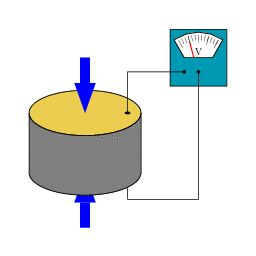
\includegraphics[width=.8\linewidth]{images/压力传感器.jpg}
            \end{figure}
        \end{minipage}
\end{frame}

% 一、压电压力传感器
% 压电式压力传感器大多是利用正压电效应制成的。正压电效应是指：当晶体受到某固定方向外力的作用时，内部就产生电极化现象，同时在某两个表面上产生符号相反的电荷；当外力撤去后，晶体又恢复到不带电的状态；当外力作用方向改变时，电荷的极性也随之改变；晶体受力所产生的电荷量与外力的大小成正比。
% 二、压阻压力传感器
% 压阻压力传感器主要基于压阻效应（Piezoresistive effect）。压阻效应是用来描述材料在受到机械式应力下所产生的电阻变化。不同于上述压电效应，压阻效应只产生阻抗变化，并不会产生电荷。
% 大多数金属材料与半导体材料都被发现具有压阻效应。其中半导体材料中的压阻效应远大于金属。
% 压阻压力传感器一般通过引线接入惠斯登电桥中。平时敏感芯体没有外加压力作用，电桥处于平衡状态（称为零位），当传感器受压后芯片电阻发生变化，电桥将失去平衡。若给电桥加一个恒定电流或电压电源，电桥将输出与压力对应的电压信号，这样传感器的电阻变化通过电桥转换成压力信号输出。
% 三、电容式压力传感器
% 电容式压力传感器是一种利用电容作为敏感元件，将被测压力转换成电容值改变的压力传感器。这种压力传感器一般采用圆形金属薄膜或镀金属薄膜作为电容器的一个电极，当薄膜感受压力而变形时，薄膜与固定电极之间形成的电容量发生变化，通过测量电路即可输出与电压成一定关系的电信号。

\begin{frame}
    \frametitle{光传感器}
    光电倍增管将微弱光信号转换成电信号，常用在光学测量仪器和光谱分析仪器中。
    \begin{figure}[htpb]
        \centering
        
\includegraphics[width=.7\linewidth]{光电倍增管}
    \end{figure}
\end{frame}


\begin{frame}
    \frametitle{图像传感器}
    \begin{figure}[htpb]
        \centering
        \setcounter{subfigure}{0}
        \subfloat[]{
\includegraphics[height=4cm]{A7RV}}\quad
        \subfloat[手机传感器VS相机传感器]{
\includegraphics[height=4cm]{手机VS相机}}
    \end{figure}
\end{frame}


\begin{frame}
    \frametitle{图像传感器}
    \begin{figure}[htpb]
        \centering
        \setcounter{subfigure}{0}
        \subfloat[CMOS尺寸]{
\includegraphics[height=4cm]{CMOS尺寸}}\quad
        \subfloat[手机CMOS尺寸]{\includegraphics[height=4cm]{手机CMOS}}
    \end{figure}
\end{frame}


% \begin{frame}
%     \frametitle{核酸检测原理}
%     \begin{figure}[htpb]
%         \centering
%         
\includegraphics[width=\linewidth]{新冠病毒检测}
%     \end{figure}
% \end{frame}


\begin{frame}
    \frametitle{声波传感器}
    \begin{minipage}{0.58\linewidth}
        声音传感器的作用相当于一个话筒（麦克风）。

    该传感器内置一个对声音敏感的电容式驻极体话筒。声波使话筒内的驻极体薄膜振动，导致电容的变化，而产生与之对应变化的微小电压。这一电压随后被转化成0-5V的电压，经过A/D转换被数据采集器接收，并传送给计算机。
    \end{minipage}\hfill
    \begin{minipage}{0.38\linewidth}
        \begin{figure}[htpb]
            \centering
            
\includegraphics[width=\linewidth]{声波}
        \end{figure}
    \end{minipage}
\end{frame}


\begin{frame}
    \frametitle{磁传感器}
    \begin{figure}[htpb]
        \centering
        \only<1>{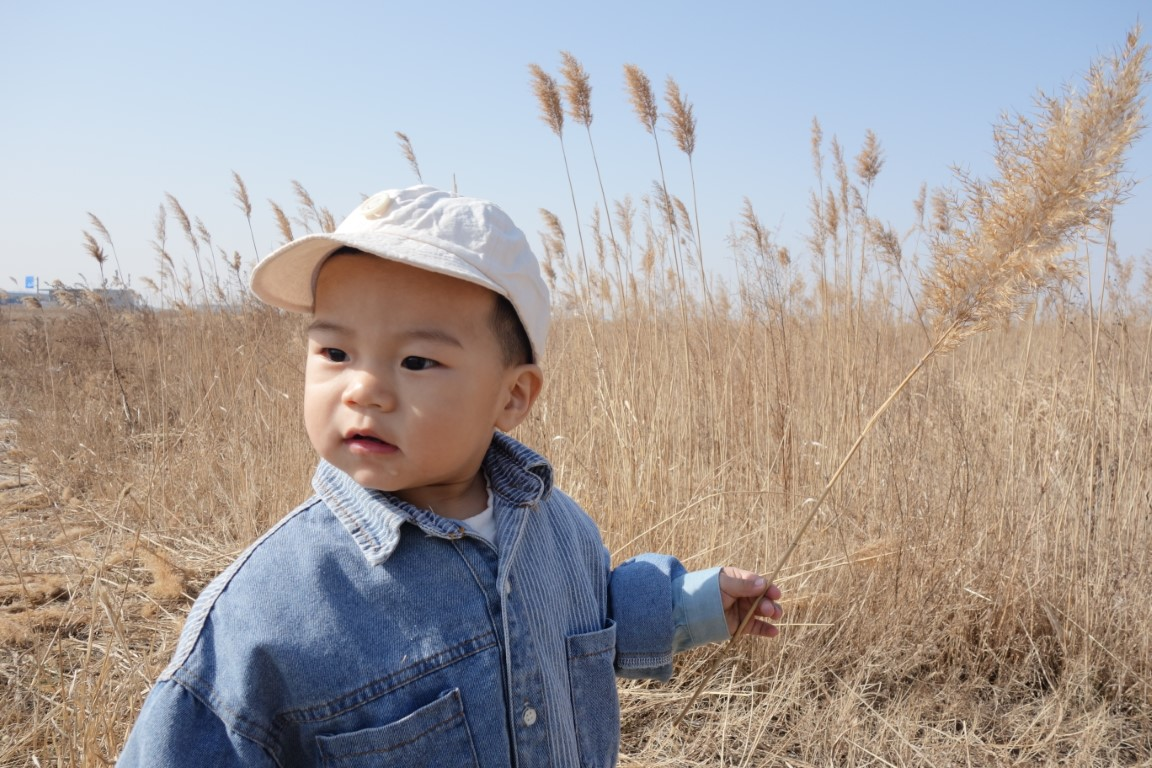
\includegraphics[height=.44\textwidth]{images/张沐凡}}
        \only<2>{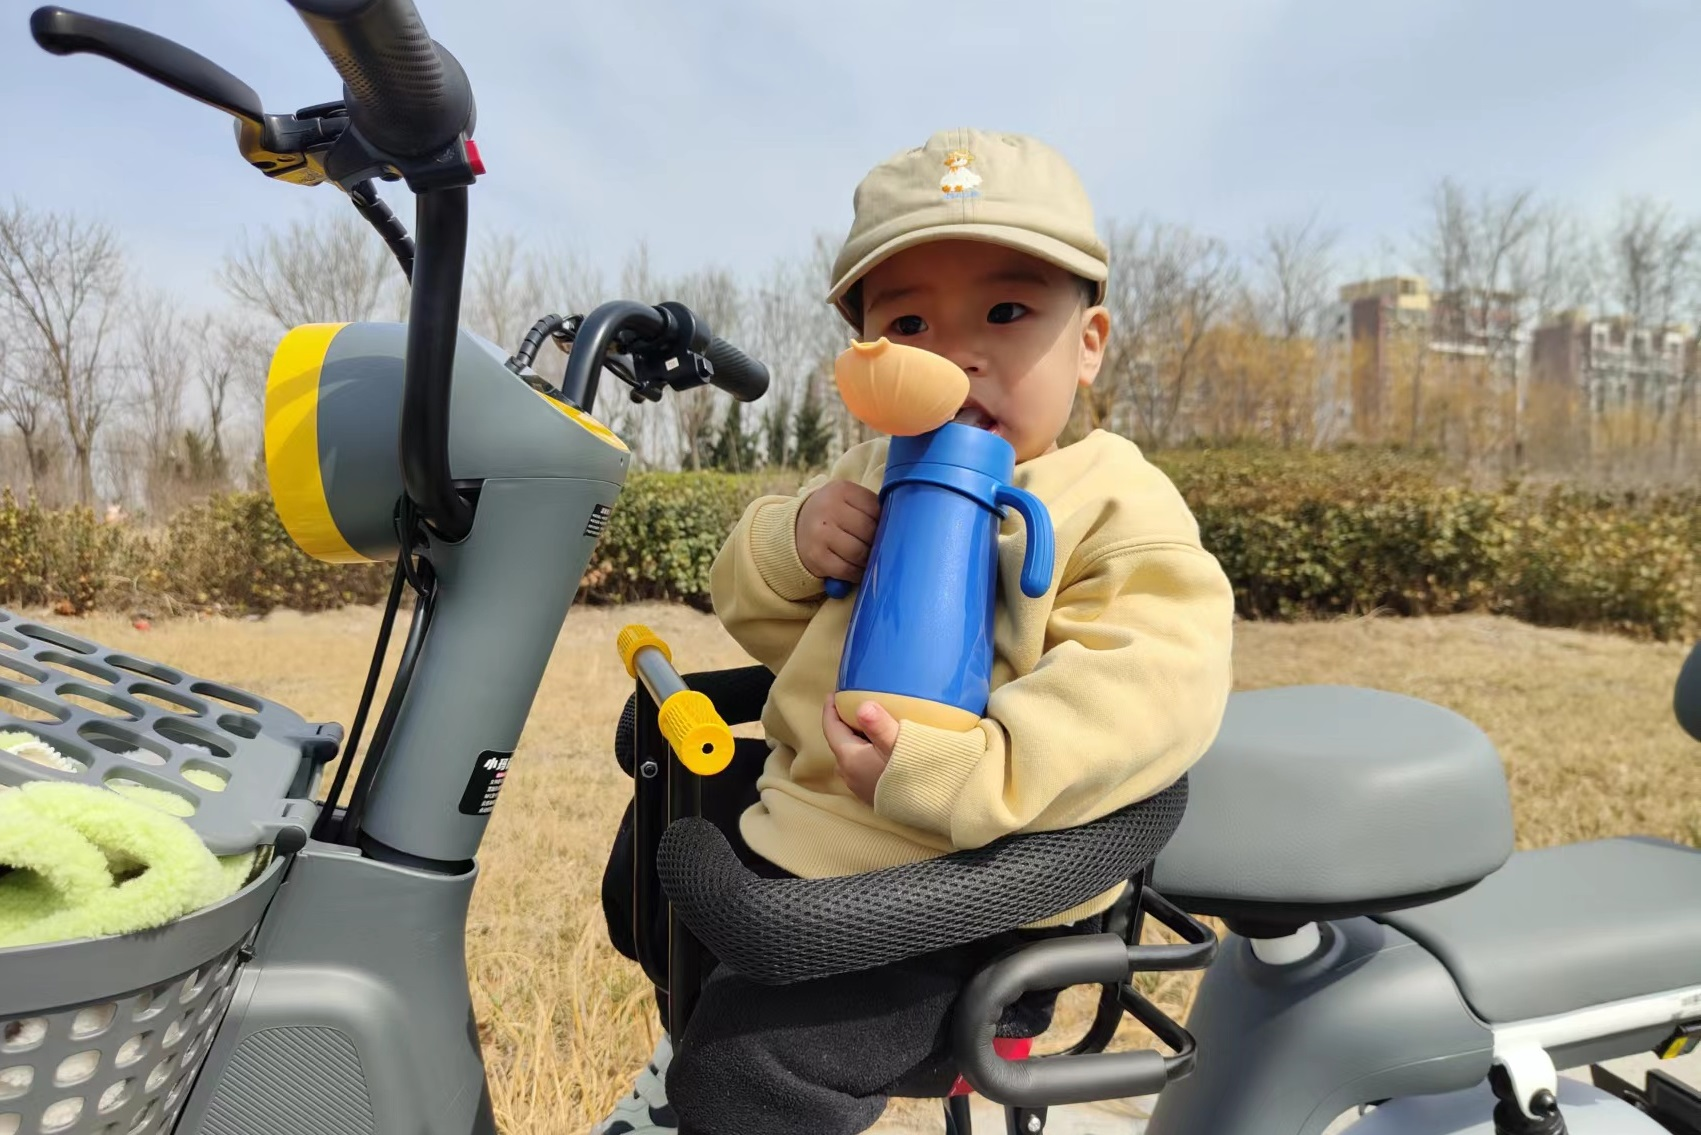
\includegraphics[height=.44\textwidth]{images/爱玛}}
        \only<3>{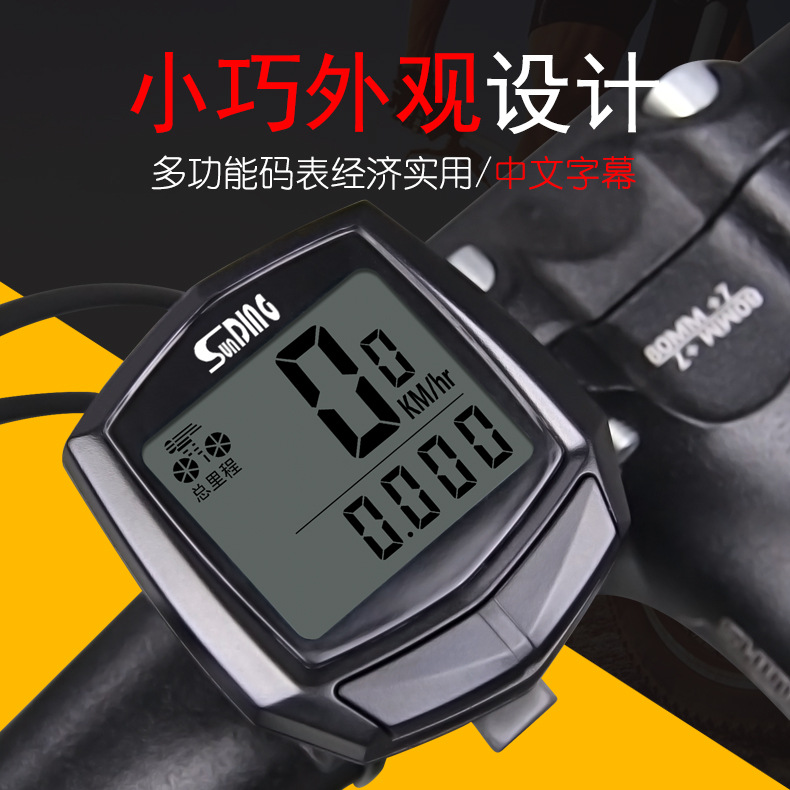
\includegraphics[height=.44\textwidth]{images/里程表.jpg} \quad 
        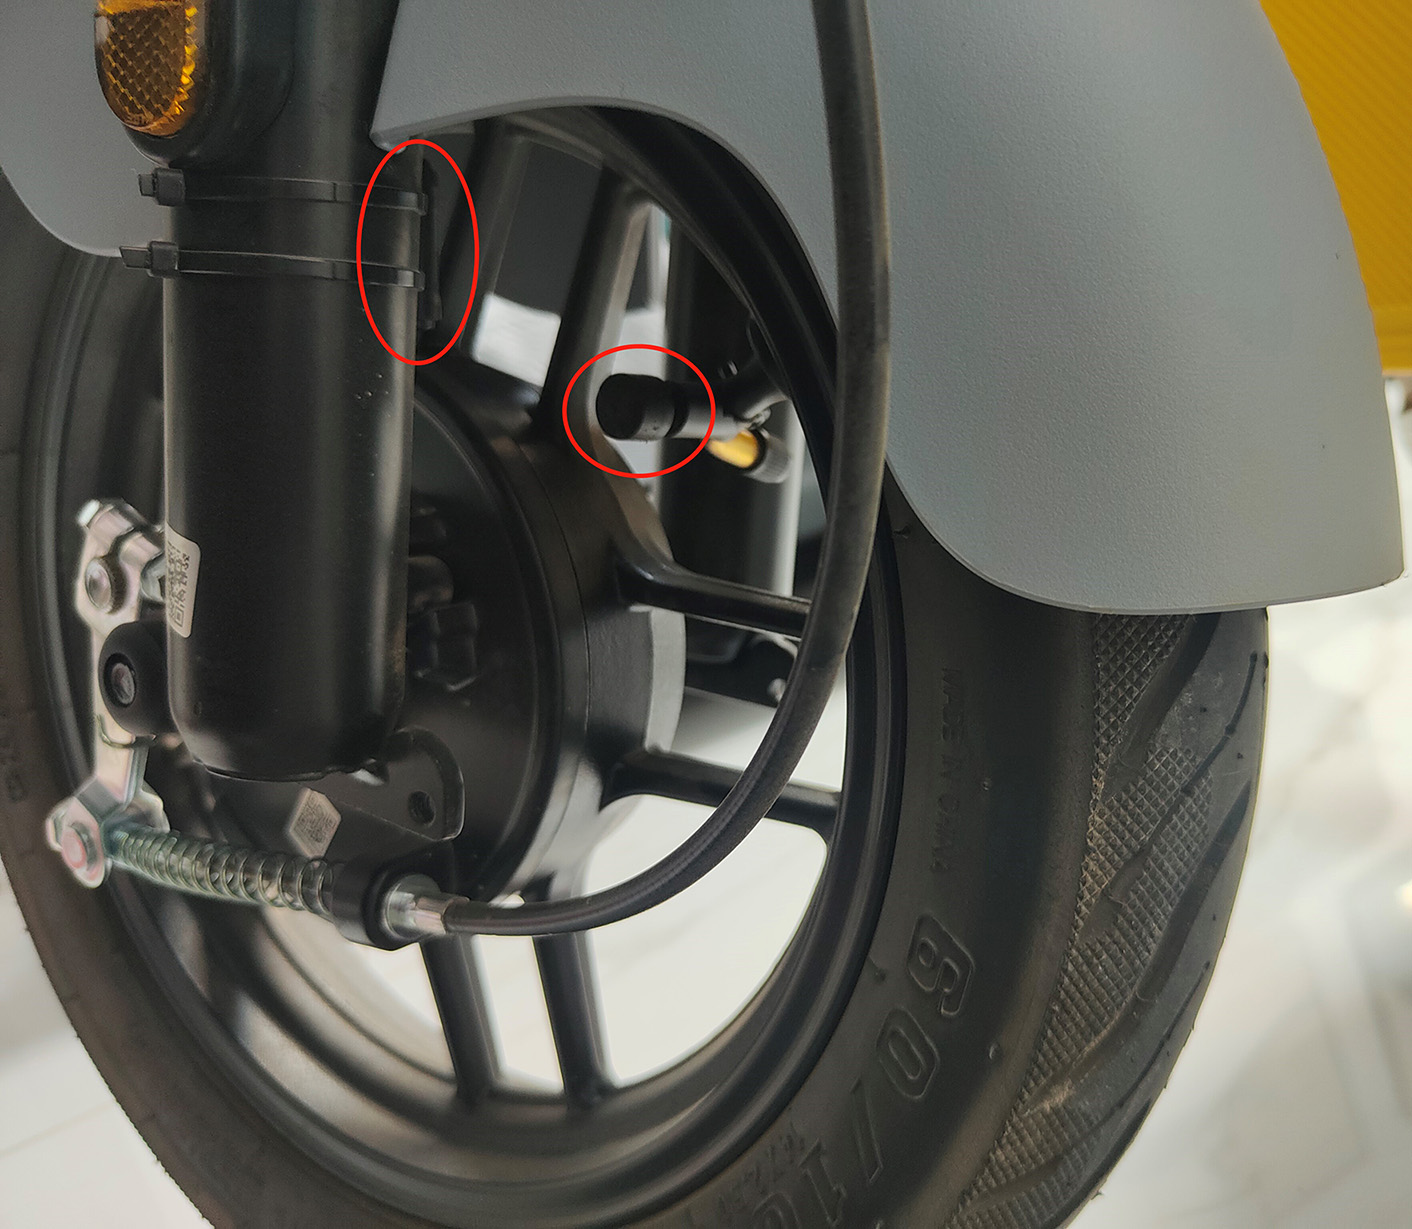
\includegraphics[height=.44\textwidth, width=.52\textwidth]{images/里程表原理3}}
    \end{figure}
\end{frame}

% \begin{frame}
%     \frametitle{磁传感器}
%     \begin{figure}[htpb]
%         \centering
%         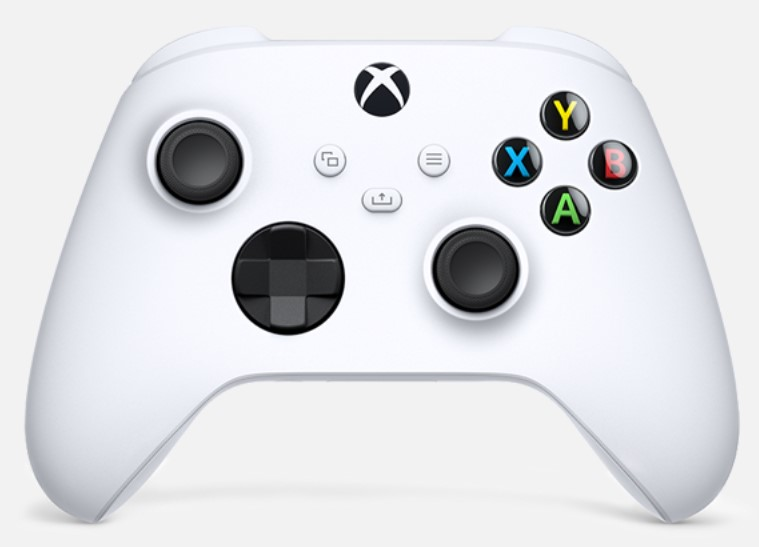
\includegraphics[height=.22\textwidth]{images/XBOX手柄}
%         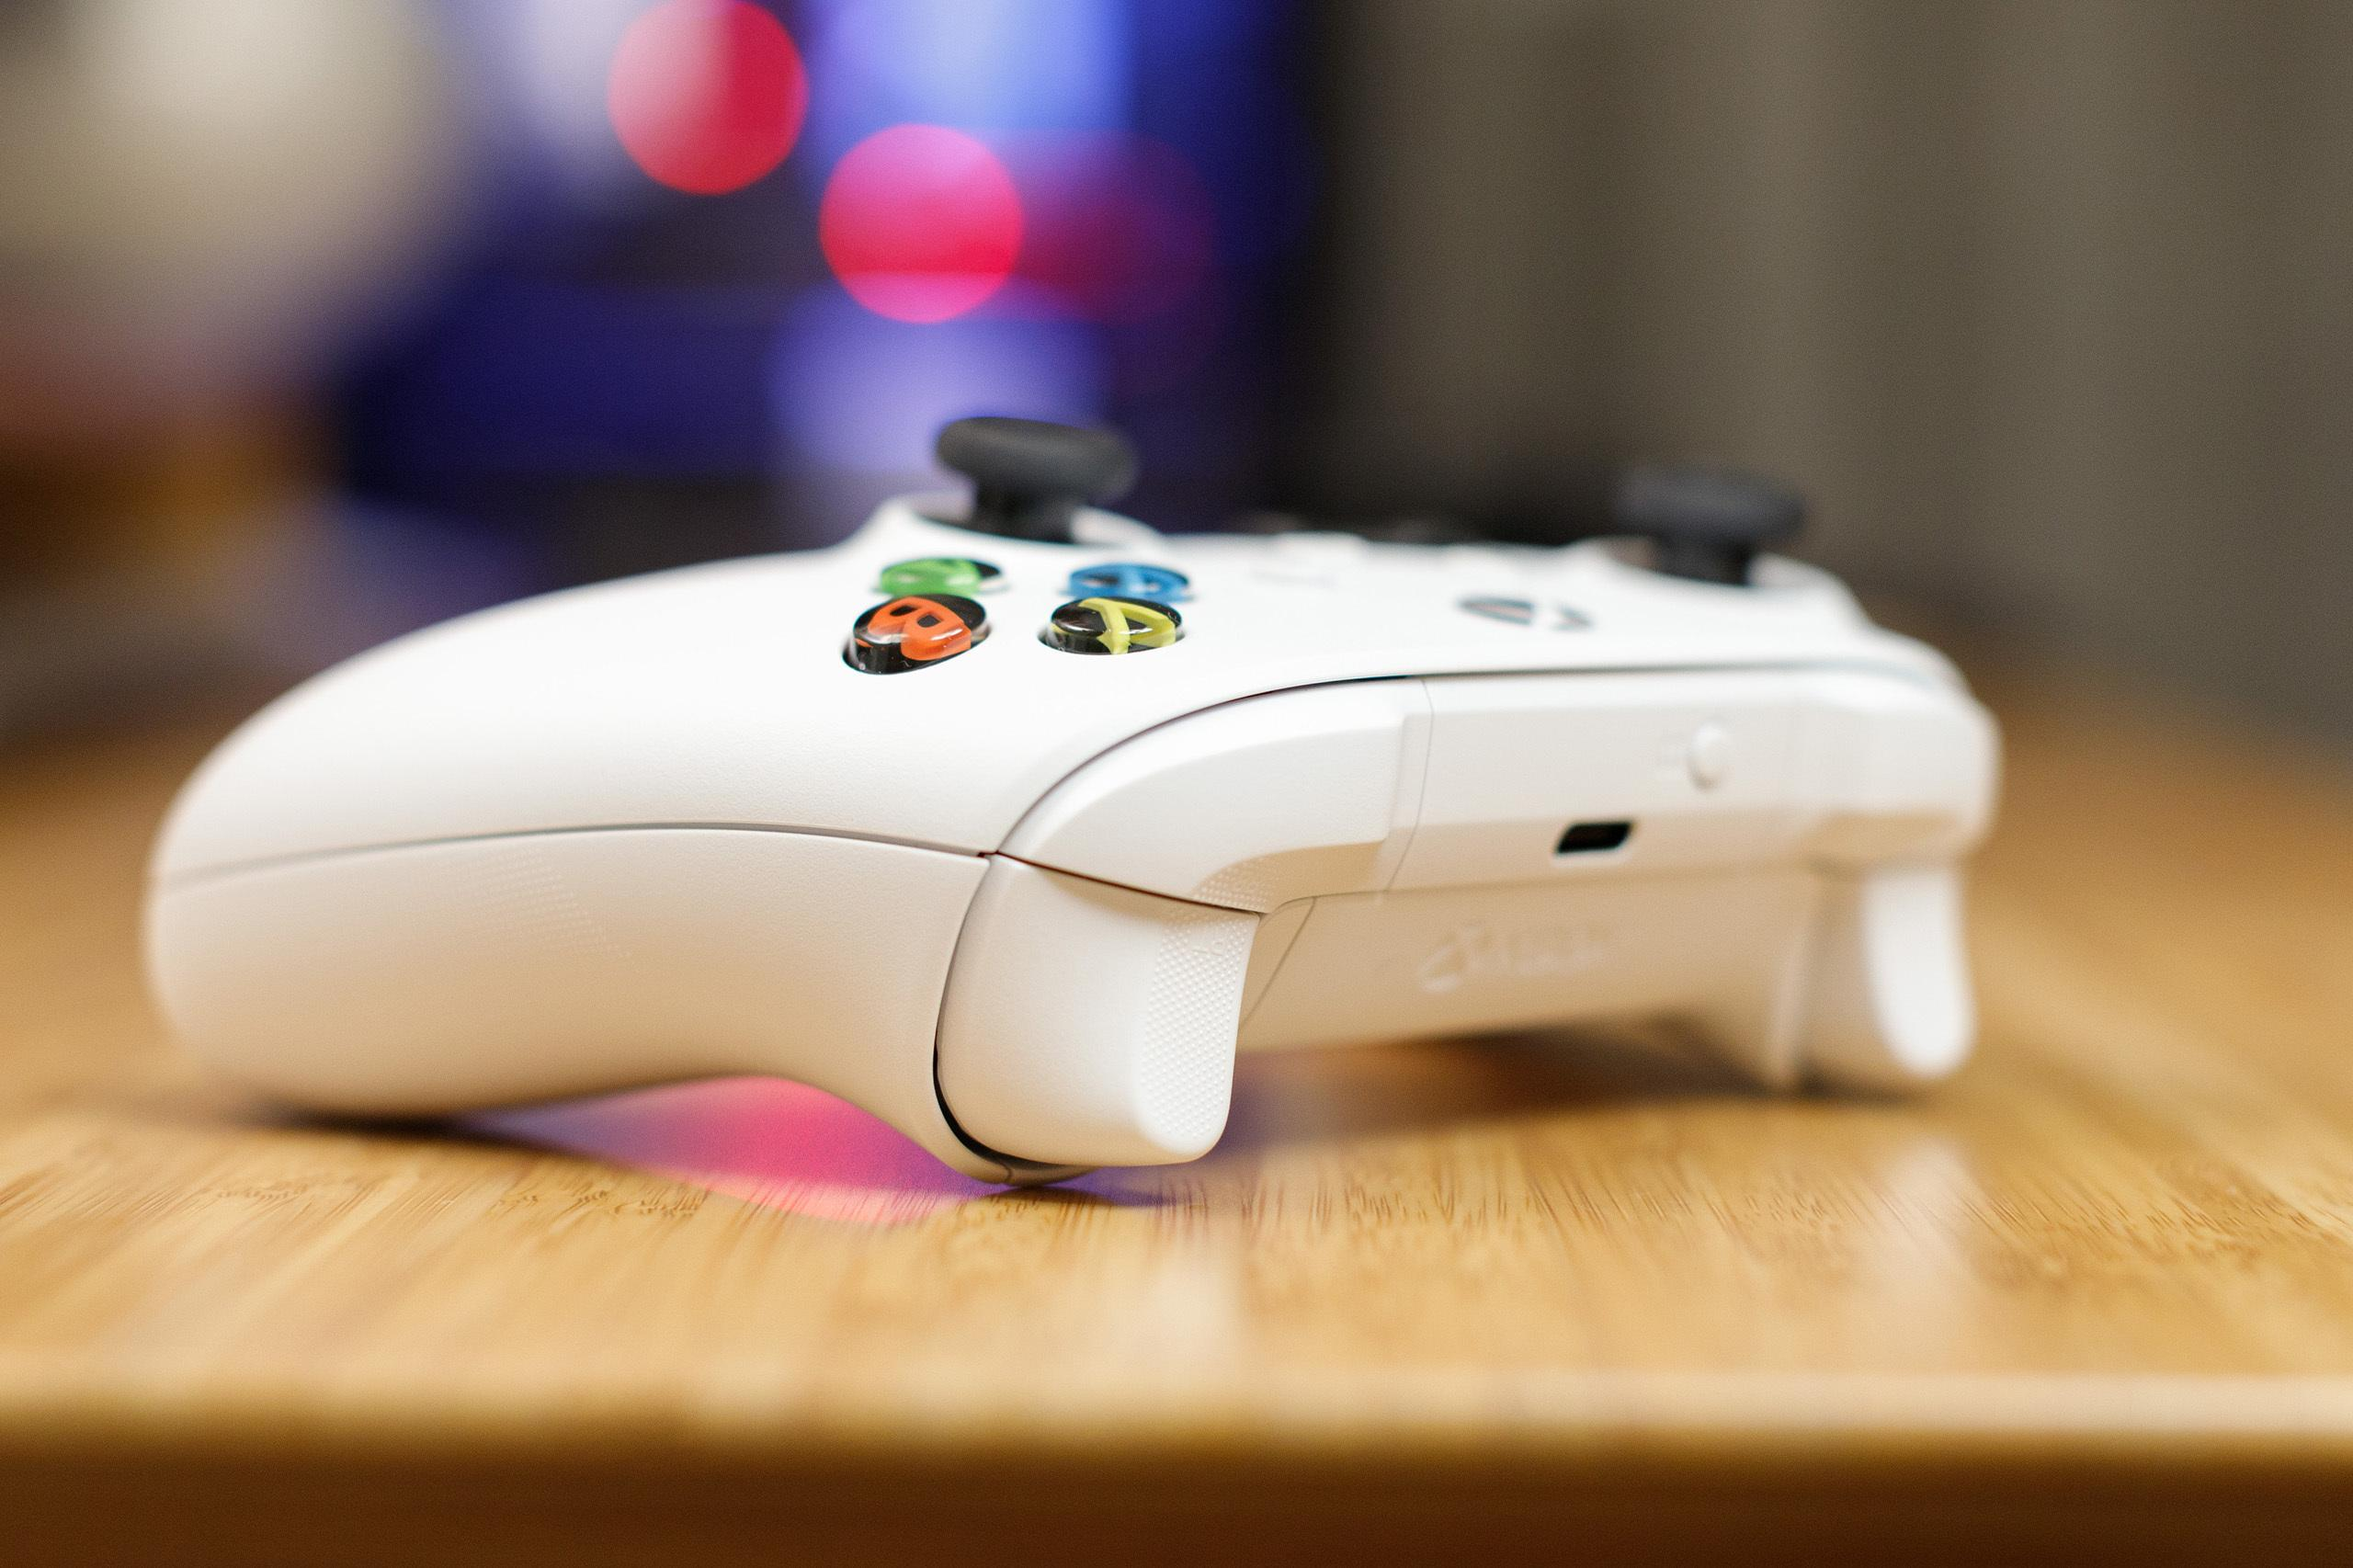
\includegraphics[height=.22\textwidth]{images/XBOX手柄扳机}
%         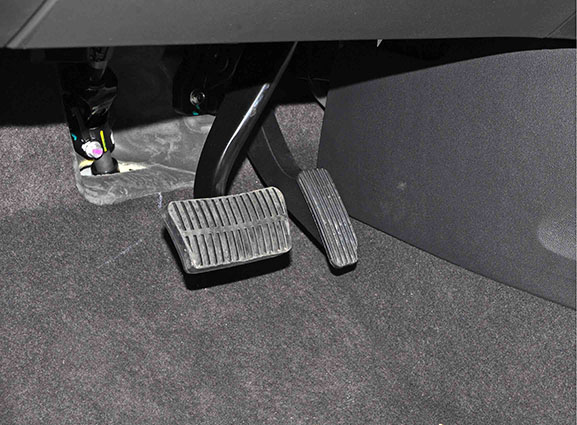
\includegraphics[height=.22\textwidth]{images/油门}
%         
\includegraphics[height=.22\textwidth]{images/GTR}
%         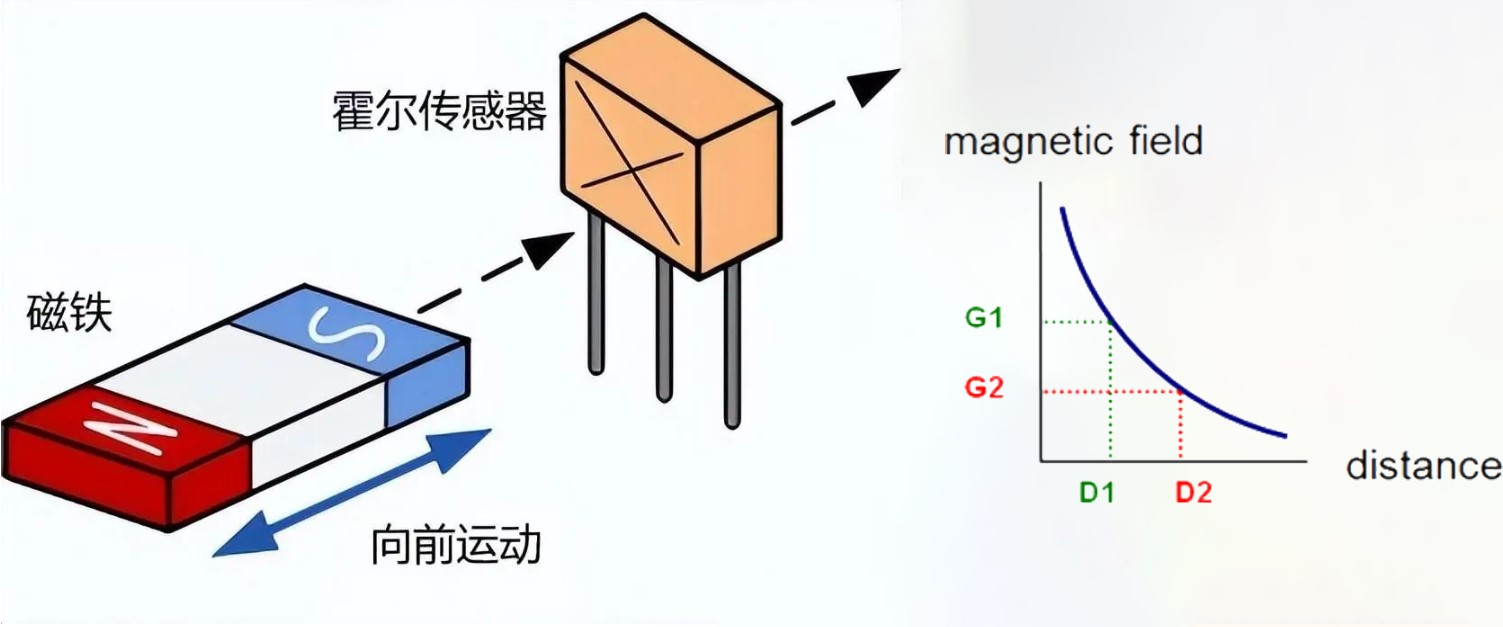
\includegraphics[height=.22\textwidth, width=.558\textwidth]{images/霍尔效应}
%     \end{figure}
% \end{frame}

% \begin{frame}
%     \frametitle{磁传感器}
%     \begin{figure}[htpb]
%         \centering
%         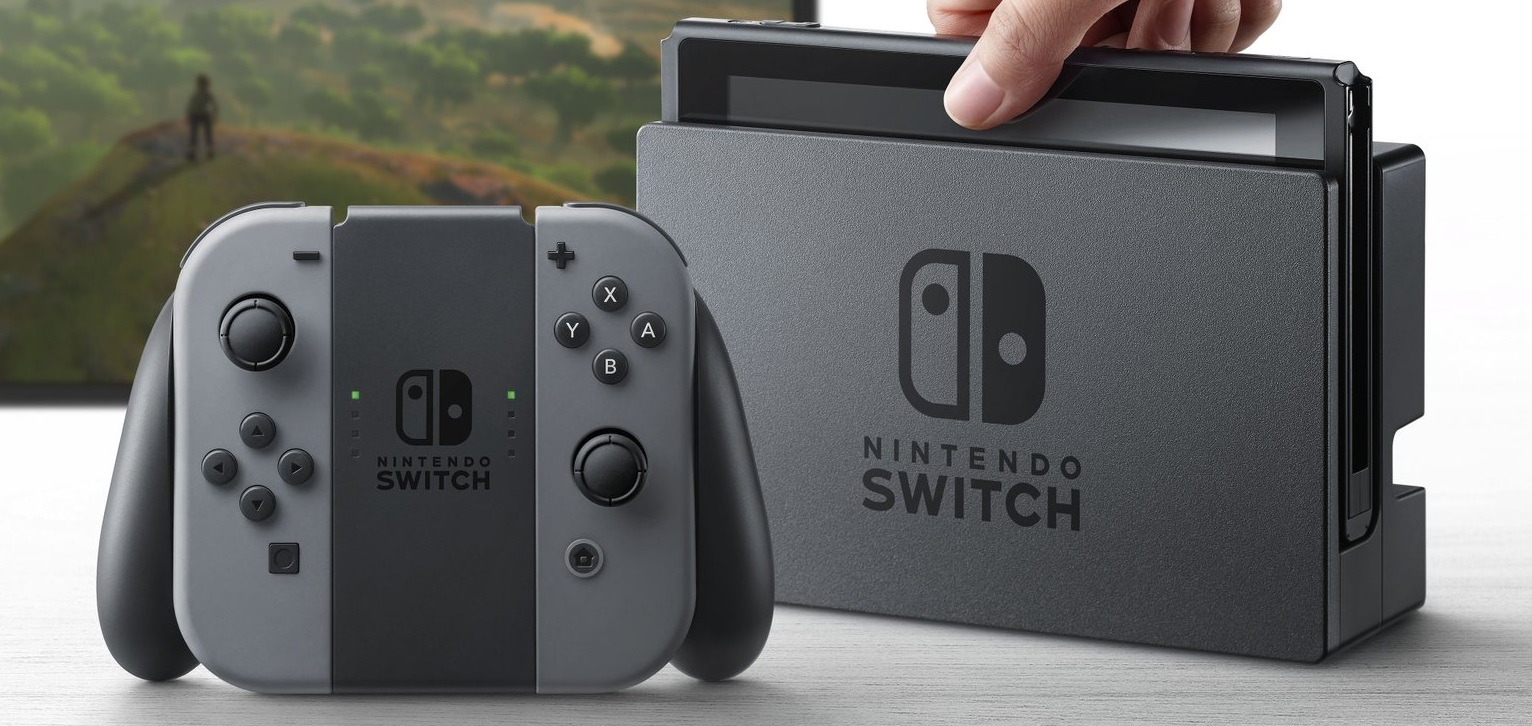
\includegraphics[height=.223\textwidth]{images/Nintendo Switch.jpg} 
%         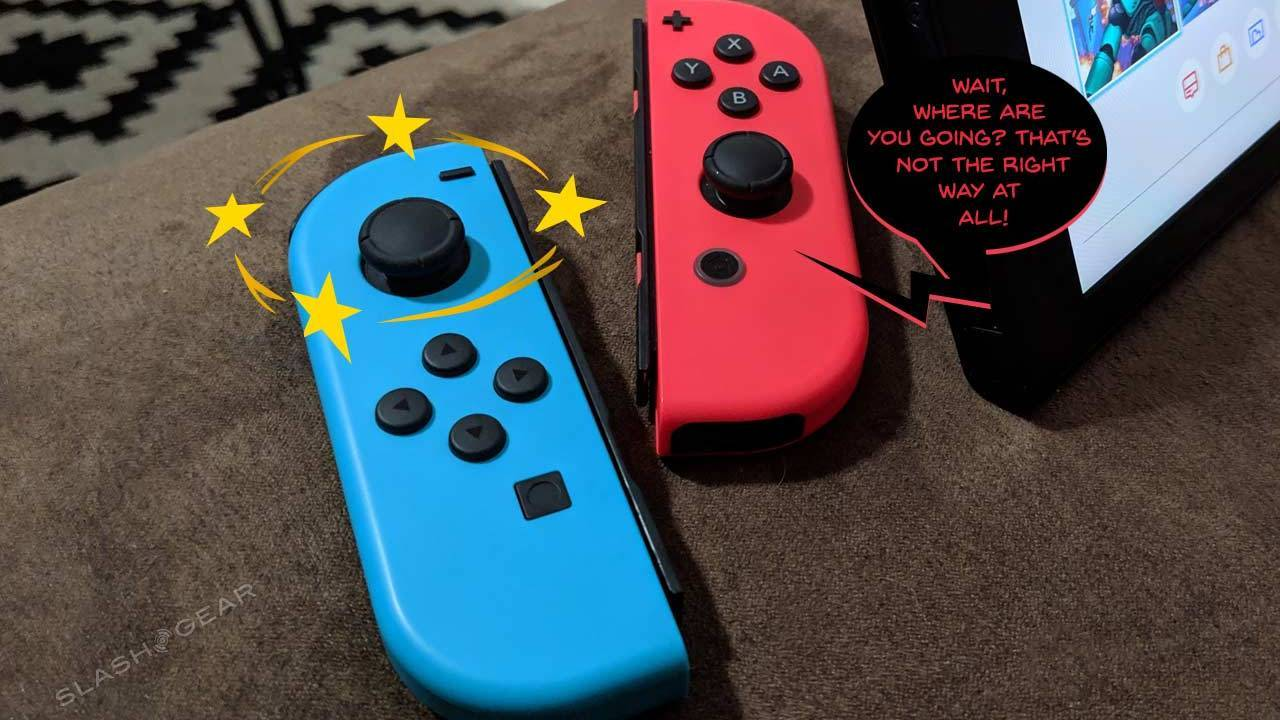
\includegraphics[height=.223\textwidth]{images/漂移}
%         \pause
%         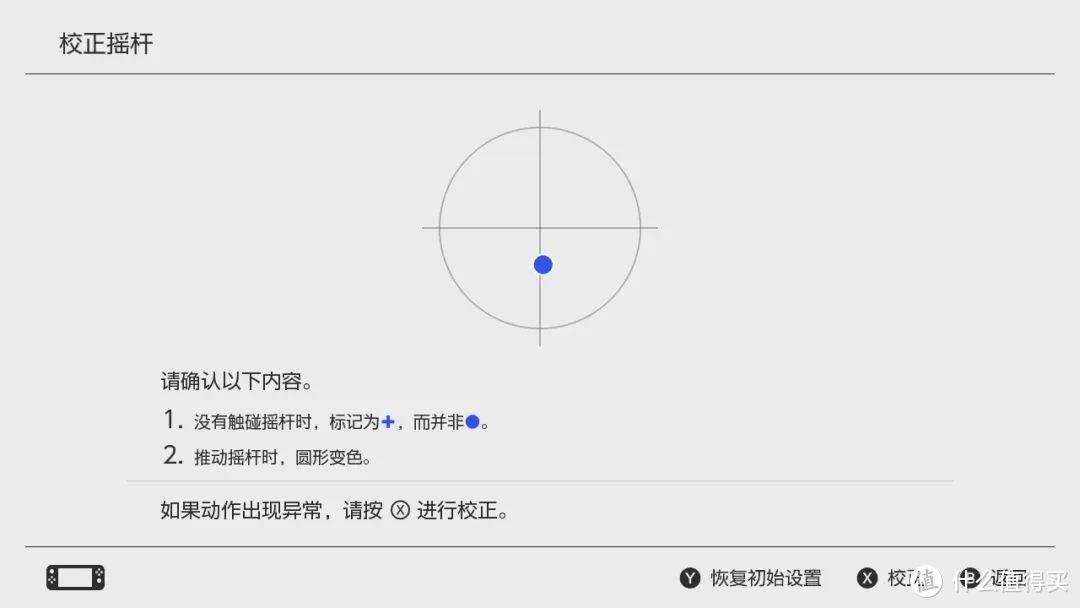
\includegraphics[height=.223\textwidth]{images/校正}
%         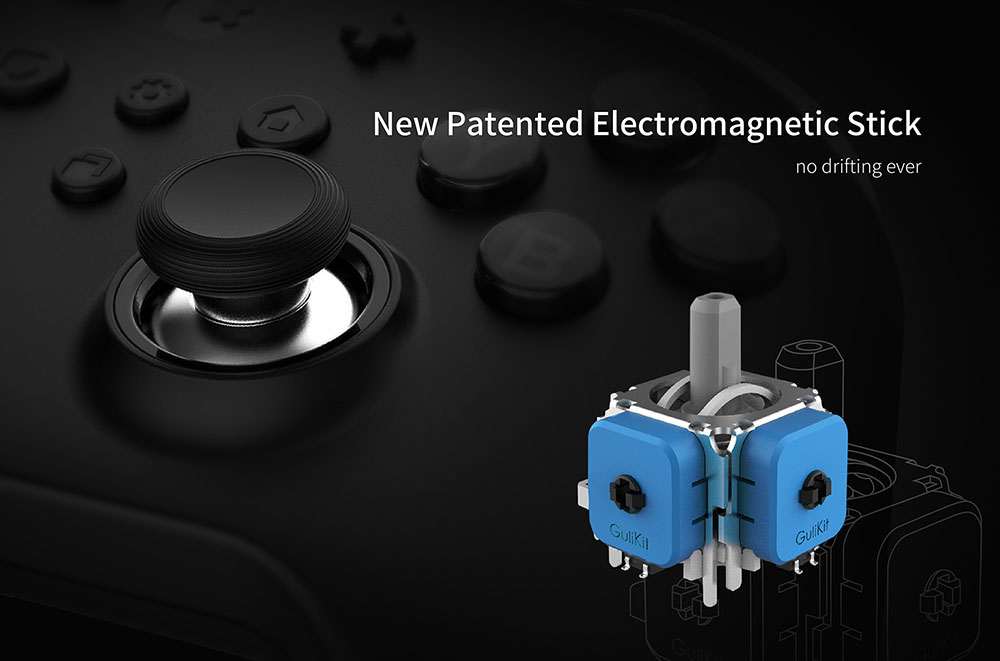
\includegraphics[height=.223\textwidth]{images/霍尔摇杆}
        
%     \end{figure}
% \end{frame}




\begin{frame}
    \frametitle{气体传感器}
    \begin{figure}[htpb]
        \centering
        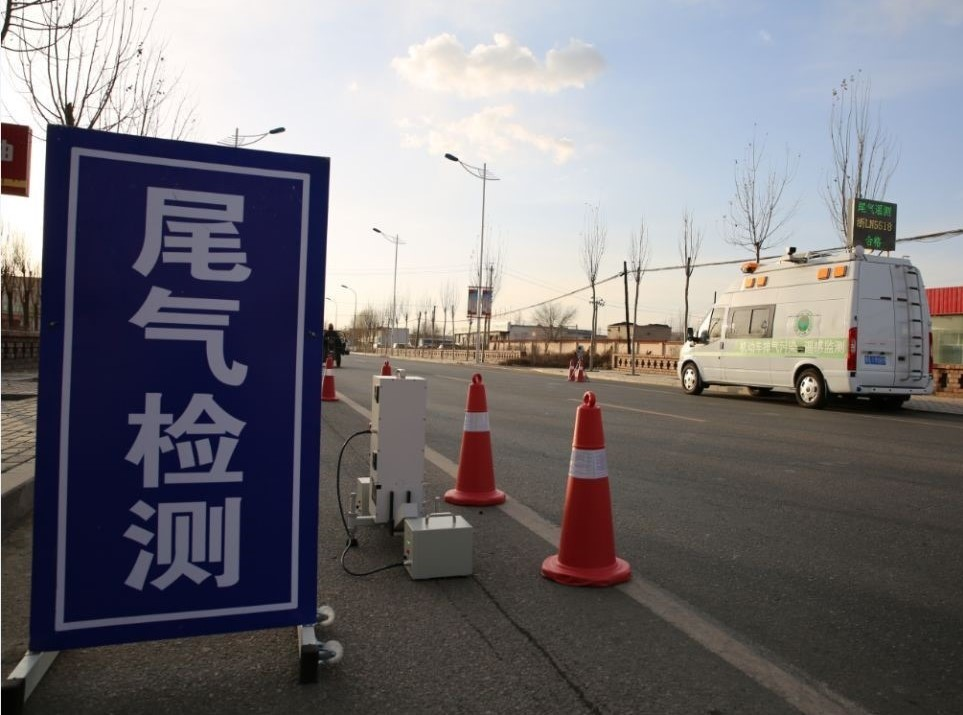
\includegraphics[height=.44\textwidth]{images/尾气监测}
    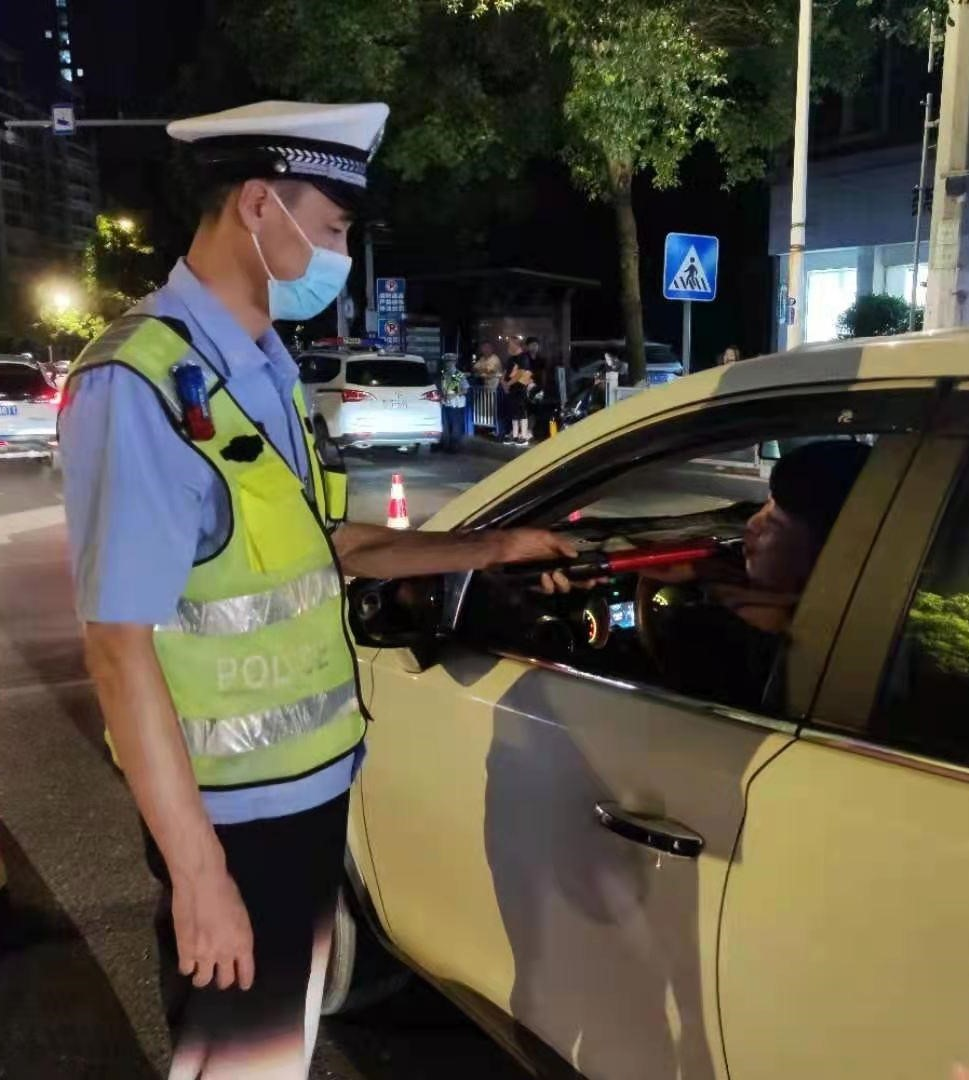
\includegraphics[height=.44\textwidth]{images/查酒驾.jpg}
    \end{figure}
    
\end{frame}

% 机动车尾气遥感监测系统对道路行驶中车辆进行尾气监测，是最有效、最经济、最方便的监测方法，监测过程快速、高效，每辆遥感车一天可监测 5000 辆以上行驶中的车辆，既不影响司机正常行驶，也不会造成交通堵塞，监测效率是人工监测的10倍以上。

% 这台移动式遥感监测车带有一套特殊的尾气遥测仪，车上配备一台电脑主机，车顶架设一面LED屏。车辆后方一台监测主机和反射单元机，摆于车道的两侧，监测仪会发出紫外光和红外光，形成光的回路。当机动车通过时，尾气中所含的一氧化碳及氮氧化物会吸收红外光、紫外光，具体数值会通过主机的换算计算出尾气中一氧化碳及氮氧化物的浓度。仪器同时还配有高速摄像机，可以对在平行范围内通过的车辆进行牌照识别，最终可以将车辆的车牌号及尾气监测结果显示在仪器屏幕上。

\begin{frame}
    \frametitle{pH传感器}
    \begin{figure}[htpb]
        \centering
        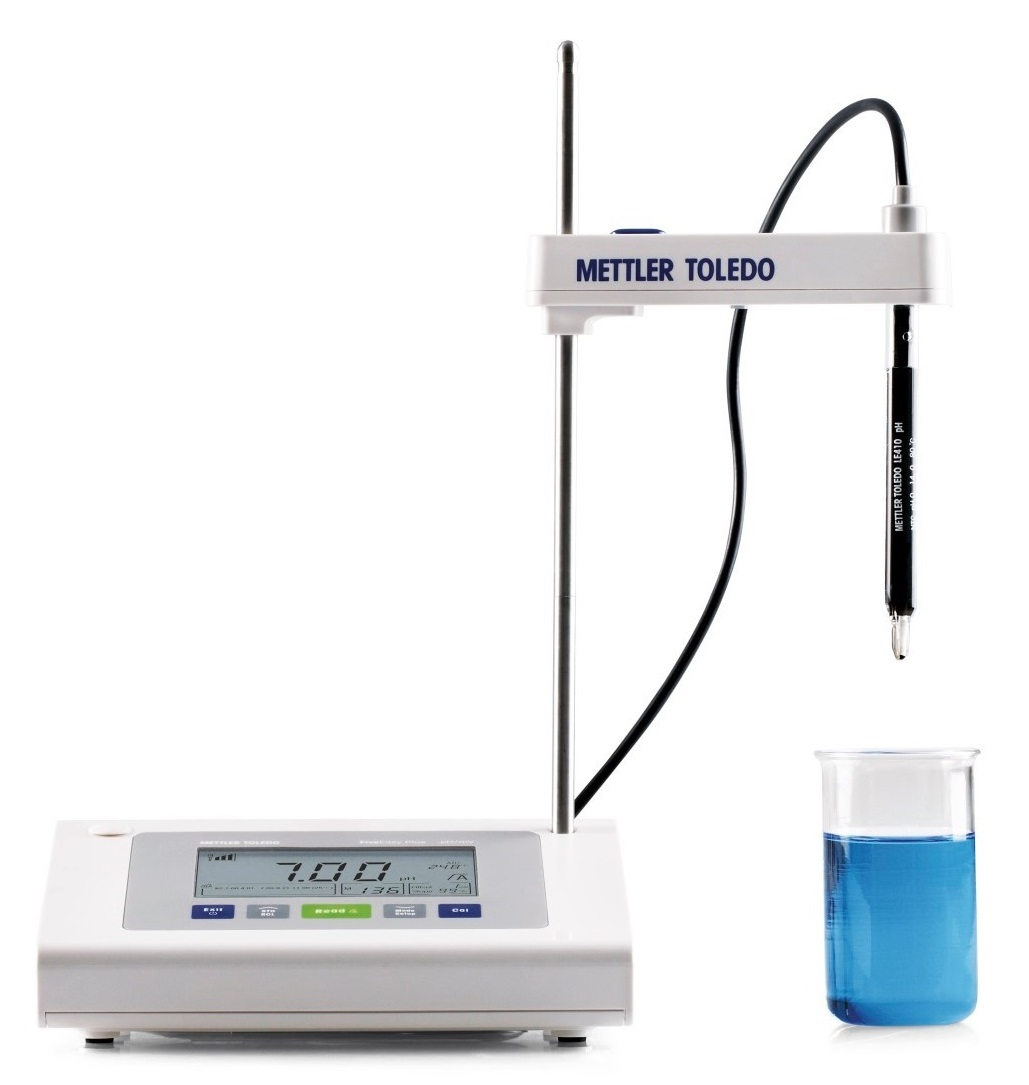
\includegraphics[height=.44\linewidth]{images/ph计.jpg} \qquad \qquad
        \includegraphics[height=.44\linewidth]{images/ph传感器}
    \end{figure}
\end{frame}
% 测量原理：
% pH传感器是由玻璃指示电极和参比电极组合在一起的复合电极。pH的测量是根据测量电极和参比电极组成的工作电池在溶液中测得的电位差，利用待测溶液的pH值与工作电池的电势大小之间的线性关系，来实现pH的在线监测。

\begin{frame}
    \frametitle{物位传感器}
    农业应用：农产品或农业生产资料的体积检测。
    \begin{figure}[htpb]
        \centering
        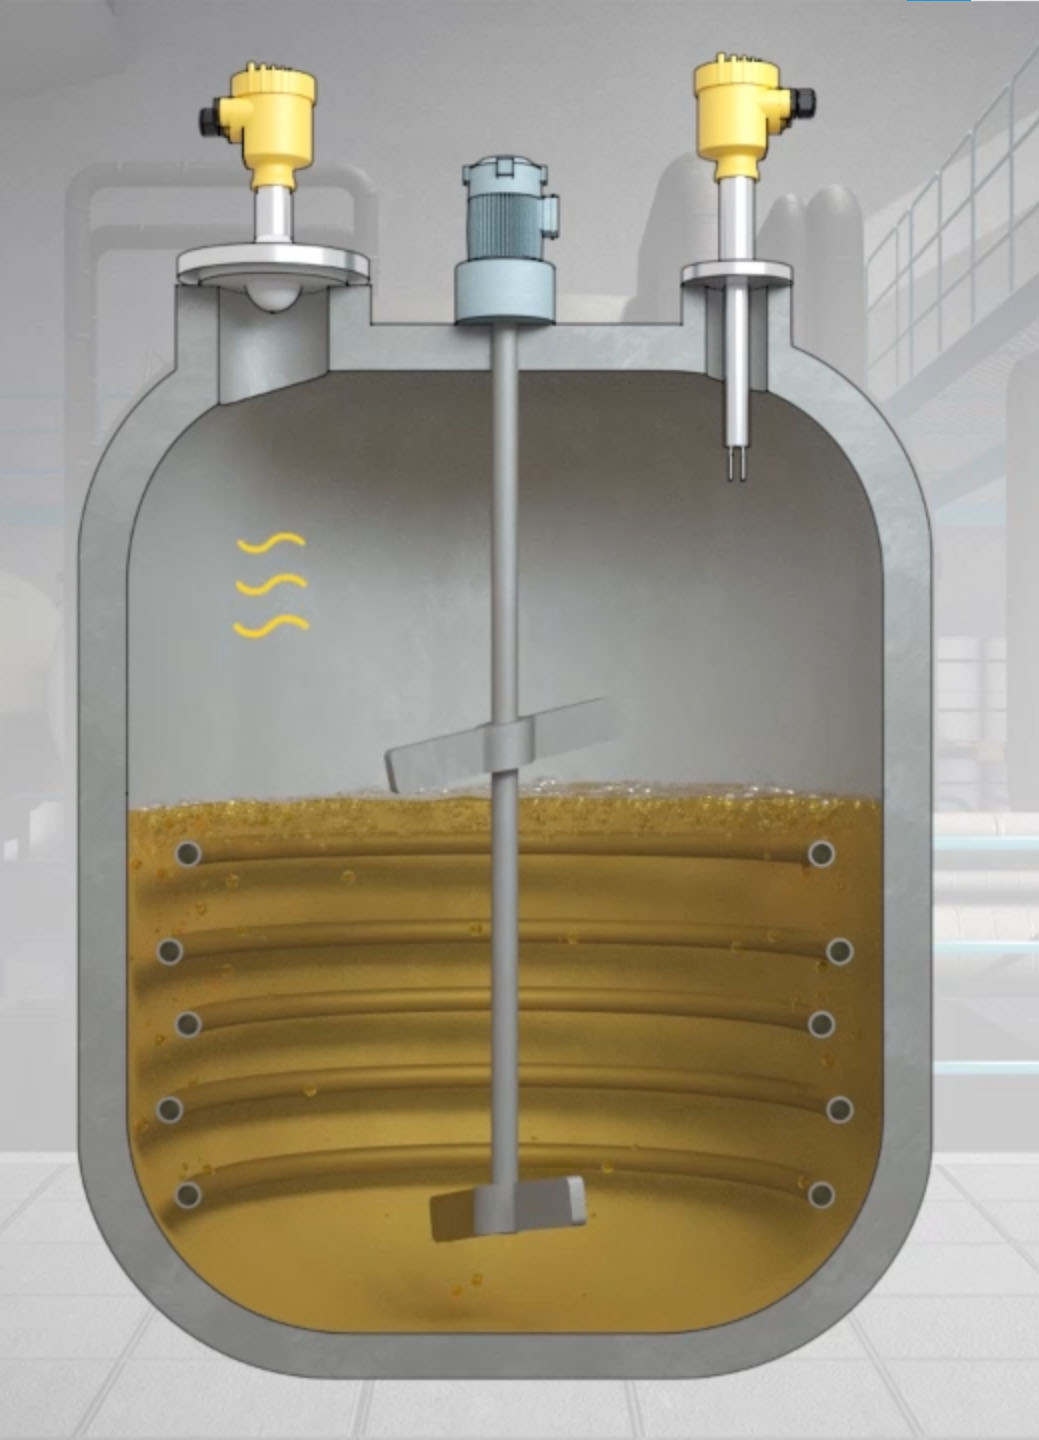
\includegraphics[height=.44\linewidth]{images/反应容器}
        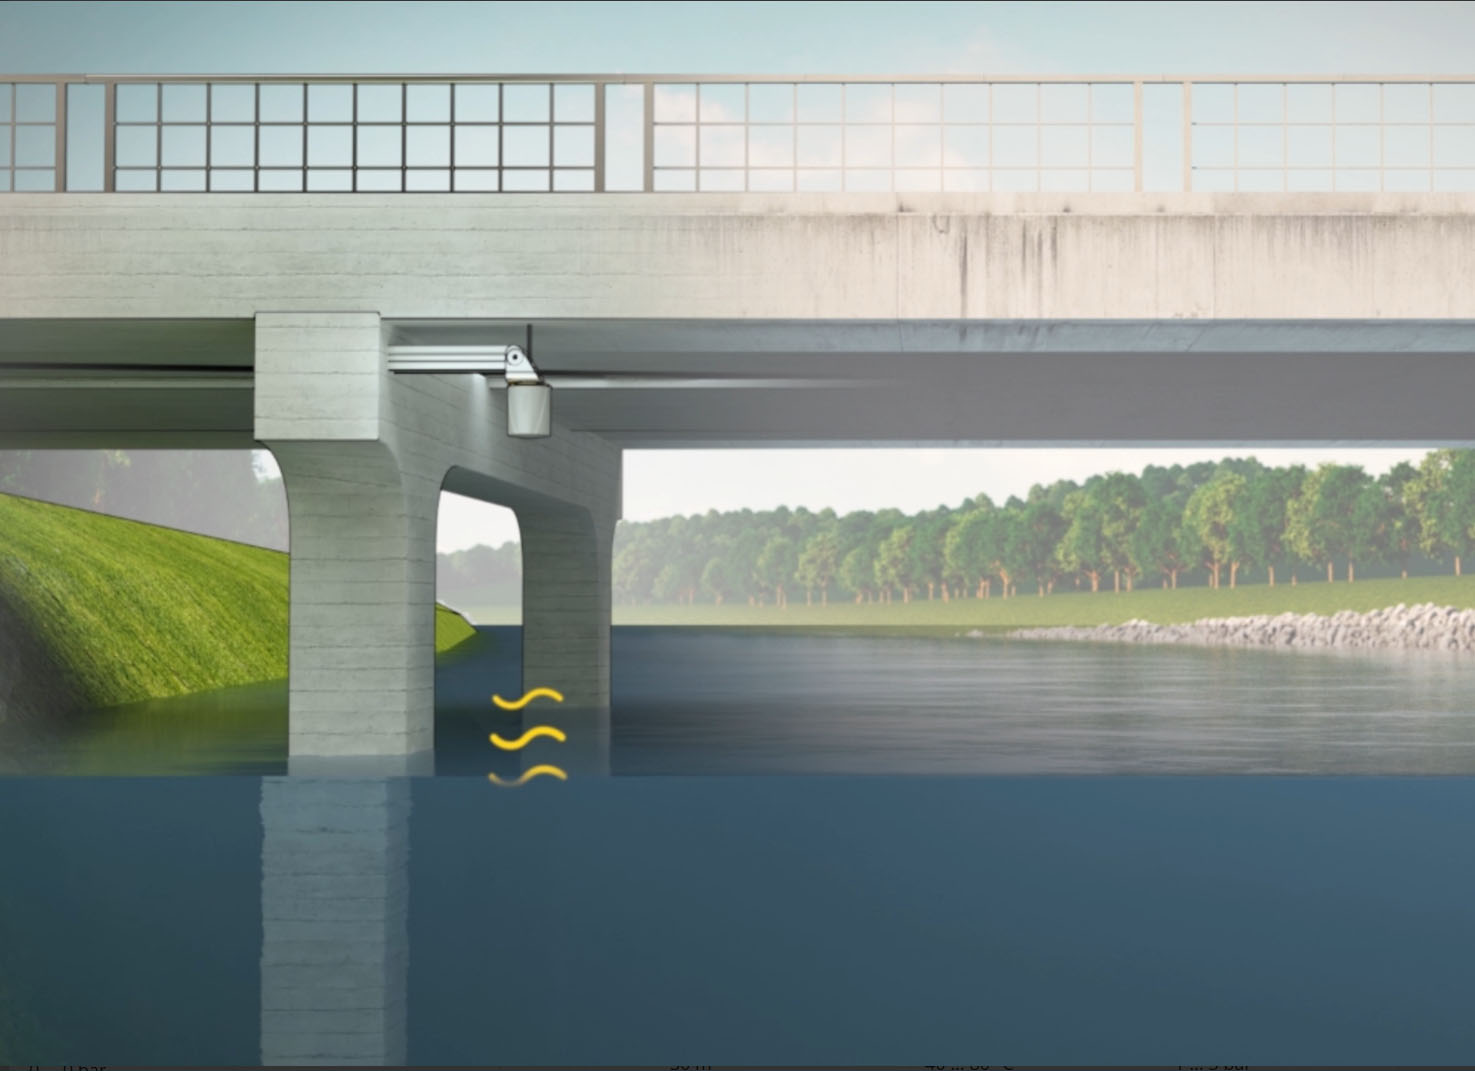
\includegraphics[height=.44\linewidth]{images/水位}
    \end{figure}
\end{frame}
% 采用无接触式超声波物位测量时，物位计朝介质的方向发出超声波脉冲，该介质又将这些脉冲反射回来。信号从发射到接收所需要的时间与容器中的物位成比例。对于简单的标准型应用，无论是在液体还是固料中，超声波物位计都是理想的测量仪表。 
% 在用雷达进行无接触式物位测量时，物位计从上方将微波信号发射给介质，该介质表面再将之反射。根据接收到的信号，物位计可测得与介质之间的距离，并由此计算出准确的物位。此测量方法既适用于液体，也适用于固料。
% 与脉冲式雷达物位计类似，超声波物位计也是利用回波的反射原理，来测量物位的高度，二者的唯一区别为雷达物位计采用的是电磁波，无需传播介质，但是超声波物位计采用的是机械波，其必须借助一定介质才能进行传播，所以当介质的压力、温度、密度、湿度等条件恒定时，超声波在介质中的传播速度是一个常数。


\begin{frame}
    \frametitle{流量/流速传感器}
    测量原理：超声波，卡罗曼涡流，转数 

    农业应用：灌溉农作物时监测灌溉量。
    \begin{figure}[htpb]
        \centering
        \setcounter{subfigure}{0}
        \subfloat[电磁式流量传感器]{
\includegraphics[height=4cm]{电磁式流量传感器}}\quad
        \subfloat[涡流流量传感器]{
\includegraphics[height=4cm]{涡流流量传感器}}\quad
        \subfloat[容积式流量传感器]{
\includegraphics[height=4cm]{容积式流量传感器}}
    \end{figure}
\end{frame}


\begin{frame}
    \frametitle{振动/冲击/加速度传感器}
    测量原理：阻抗变化，静电效应，MEMS

    农业应用：农业机械运行状态检测，例如振动，加速度，角速度等
    \begin{figure}[htpb]
        \centering
        \setcounter{subfigure}{0}
        \subfloat[冲击传感器]{
\includegraphics[height=4cm]{冲击传感器}}\quad
        \subfloat[振动传感器]{
\includegraphics[height=4cm]{振动传感器}}\quad
        \subfloat[加速度传感器]{
\includegraphics[height=4cm]{加速度传感器}}
    \end{figure}
\end{frame}


\begin{frame}
    \frametitle{生物传感器}
    测量原理：酶传感器，微生物传感器，DNA传感器，细胞传感器

    农业应用：农药残留量分析、微生物和毒素的检验、食品鲜度的检测、水环境监测等

    \begin{figure}[htpb]
        \centering
        \setcounter{subfigure}{0}
        \subfloat[农药残留检测]{
\includegraphics[height=4cm]{农药残留检测}}\quad
        \subfloat[食品检测]{
\includegraphics[height=4cm]{食品检测}}\quad
        \subfloat[水质监测]{
\includegraphics[height=4cm]{水质监测}}
    \end{figure}
\end{frame}


\begin{frame}
    \frametitle{智能手表/手环中的传感器}
        \begin{minipage}{0.3\linewidth}
            \begin{figure}[htpb]
                \centering
                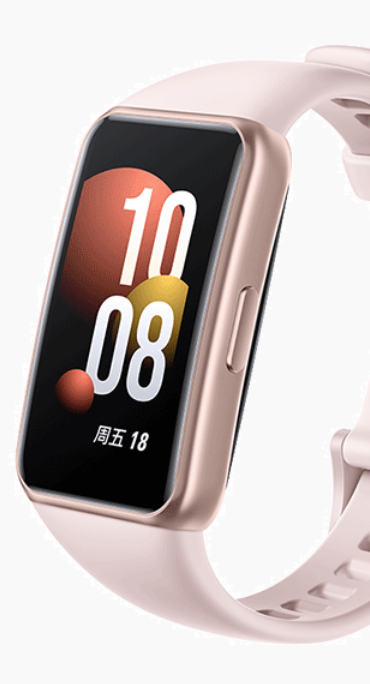
\includegraphics[height= 200pt]{images/手环7}
            \end{figure}
        \end{minipage}\hfill
        \begin{minipage}{0.68\linewidth}
            
            $\vcenter{\hbox{
\includegraphics[height= 25pt]{images/抬腕亮屏}}}$ {\bfseries 抬腕亮屏} \qquad 加速度传感器、陀螺仪

            \bigskip
            $\vcenter{\hbox{
\includegraphics[height= 25pt]{images/记步}}}$ {\bfseries 记步} \qquad \qquad 加速度传感器

            \bigskip
            $\vcenter{\hbox{
\includegraphics[height= 25pt]{images/心率}}}$ {\bfseries 心率} \qquad \qquad 光学心率传感器、生物电阻抗传感器

            \bigskip
            $\vcenter{\hbox{
\includegraphics[height= 25pt]{images/血氧}}}$ {\bfseries 血氧} \qquad \qquad 光学传感器

            \bigskip
            $\vcenter{\hbox{
\includegraphics[height= 25pt]{images/睡眠}}}$ {\bfseries 睡眠监测} \qquad 加速度传感器、心率传感器
        \end{minipage}
    
\end{frame}

% 抬腕亮屏：通过加速度传感器和陀螺仪检测手环状态，还会涉及一些复杂的算法，因为抬腕亮屏不仅要判断手环的位置、表盘朝向变化，还要综合考虑其他因素，保证检测到的是真的“抬腕”，从而避免不必要的亮屏耗电。
% 记步：重力加速度传感器。通过获取三个方向的加速度来获取加速度数据。对于加速度数据进行分析，判断是否为正常行走类型（包括前进，后退，上楼，下楼，跑步等类型）。通过以上数据，计算出当前使用者的步长，最终统计出行走时间，距离，运动强度等数据。
% 心率：最常见的是光学心率传感器，原理是通过LED绿光照射紧贴传感器的皮肤和附近血管，通过测算光线被吸收的波动来判断心率状态，辅助运动检测，也可以检测心脏异常，及时反馈报警。血液之所以呈现红色，是因为它反射红光并吸收绿光。心脏跳动时，流经手腕的血流量会增加，吸收的绿光也会增加；在心跳间隔期间减少。
% 心率2：另一种电极式心率传感器。电极可以在与“心率”App 或移动心电图房颤提示软件搭配使用时测量通过你心脏的电信号，经过峰值检测可以获得心率。当你将手指放在数码表冠上时，就会在你的心脏和双臂之间形成一个闭合电路，从而捕捉到通过你胸部的电脉冲。https://support.apple.com/zh-cn/HT204666
% 血氧:光学传感器。原理与心率检测一致，都是通过背面贴近皮肤的模块发射光线，利用光敏电阻检测被血液吸收一部分的光线波动来分析血氧状态，不同的是这个过程发出的光线往往是红外光，而且容易受到各种因素干扰，因此手环/手表上的血氧检测准确度有限，只能作为参考。​
% 睡眠监测：主要靠心率传感器、加速度传感器来实现。简单来说，人在清醒状态和睡眠状态的心率有很大的差别，加速度传感器能有效监测人的位移变量，就是监测你的动作，人在入睡的时候，手肯定不会有较大的垂直高度位移。当我们处于睡眠状态的时候，心率一般情况下会下降；而当用户睡得很深的时候，心率会下降的更低。而手环通过监测我们的一个心率变异性，从而来判断我们的睡眠时间和睡眠的深浅。
